\chapter{Introduction}
\label{Chapter1}

%------------------------------------------------------------------------------

\section{Introduction}

Surveillance cameras have become popular and placed almost everywhere, e.g. train stations, airports, banks, shops, streets. The balance between security and privacy is an active subject for political/social debates. It is hard to keep a balance between security and privacy, a person may feel protected when he knows himself and his surroundings are being observed, but at the same time he may feel uncomfortable.

The information that a person probably wants to know most about surveillance cameras is probably their viewing fields, e.g. where the cameras are, whether he is inside the observed area. For indoor environment, because the space is usually small, people may easily locate the position and estimate the viewing fields of the cameras. For outdoor environment, it is almost impossible to find surveillance camera systems which support people to visually know the viewing fields in real scene. Fortunately, there is a technology which can be applied for situations like this: MR (Mixed Reality). MR is the encompassing of both Augmented Reality and Augmented Virtuality, merging the real world in which we are living and the virtual world created by computers. MR produces new environments where real and virtual entities can co-exist and interact in realtime \cite{Reference3}.

MR applications are traditionally equipped with HMDs (Head Mounted Display) as shown in figure \ref{fig:HMD}. However, HMDs are usually bulky and inconvenient for outdoor applications, where wide-range mobility is crucial. In recent years, mobile devices have become popular, devices like cell phones, PDA (Personal Digital Assistants) can be seen everywhere. Their prices have come down and they could reach the hands of common people even in developing countries like Viet Nam. High-end mobile devices, such as Apple iPhone and Google T-Mobile G1, usually have high specifications. More importantly for outdoor MR applications, they are almost always equipped with built-in cameras, GPS (Global Positioning System), and accelerometer devices. These auxiliary devices usually meet the need of common outdoor MR applications because they provide video and information to help estimating position and orientation of the mobile devices \cite{Reference2} \cite{Reference4}.

\begin{figure}[htbp]
	\centering
	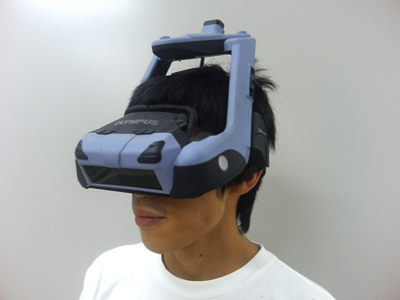
\includegraphics{./Primitives/hmd.jpg}
	\rule{35em}{0.5pt}
	\caption[An HMD]{An HMD}
	\label{fig:HMD}
\end{figure}

However, image processing applications usually need large memory and powerful computing capability. Even current high-end cell phones and PDAs may not run MR applications properly without special program optimizations. For compute-intensive outdoor MR applications, more powerful UMPCs (Ultra-Mobile Portable Computer) like the one in figure \ref{fig:VAIO} may be used. UMPCs equipped with built-in camera, GPS, and gyrocompass devices have been found practical and are a topic of many researches \cite{Reference2} \cite{Reference4} \cite{Reference13}.

\begin{figure}[htbp]
	\centering
	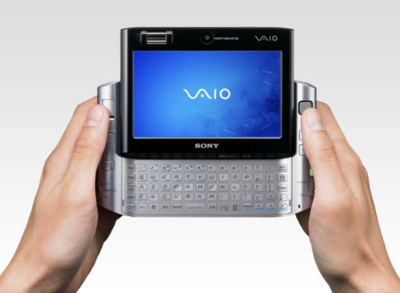
\includegraphics{./Primitives/vaio.png}
	\rule{35em}{0.5pt}
	\caption[Sony VAIO VGN-UX90PS with a camera at the front]{Sony VAIO VGN-UX90PS with a camera at the front (top, center)}
	\label{fig:VAIO}
\end{figure}

\begin{figure}[htbp]
	\centering
	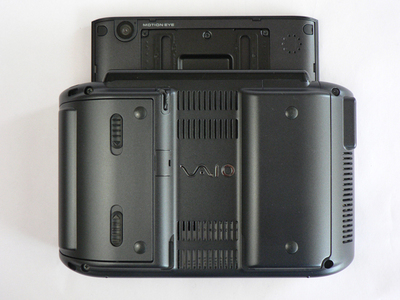
\includegraphics{./Primitives/vaio_back.jpg}
	\rule{35em}{0.5pt}
	\caption[Sony VAIO VGN-UX90PS with a camera at the back]{Sony VAIO VGN-UX90PS with a camera at the back (top, left)}
	\label{fig:VAIOBack}
\end{figure}

This research aims to visualize the viewing fields of outdoor surveillance cameras on the screen of mobile devices. In this research, we propose:

\begin{itemize}
	\item Five methods to visualize viewing fields of surveillance cameras for outdoor MR (chapter \ref{Chapter2}).
	\item A prototype based on server-side PTAM (Parallel Tracking and Mapping) \cite{Reference12} technology (chapter \ref{Chapter3}). The prototype uses a Sony VAIO VGN-UX90PS (appendix \ref{AppendixA}) and provides realtime video. Because the VAIO is still weak to do PTAM processing, we connect it wirelessly to an Apple MacBook Pro, which actually does the heavy work of PTAM. This results in a prototype providing realtime video with no requirement for any GPS or gyrocompass devices.
\end{itemize}

An experiment using the prototype to evaluate the visualization methods is described in chapter \ref{Chapter4}.

%------------------------------------------------------------------------------

\section{Use Cases}
\label{UseCases}

Using the prototype we make in chapter \ref{Chapter3}, when a user wants to see the visualized viewing fields of surrounding surveillance cameras on his own mobile device screen, the typical usage scenario is (figure \ref{fig:VAIOMacBookPro}):

\begin{enumerate}
	\item The user points the mobile camera in a certain direction.
	\item Through wireless network, the mobile device continuously sends frames captured by the camera of the scene to a more powerful remote computer for processing.
	\item Based on the frames, the remote computer estimates the position and orientation of the mobile camera, and send them to the mobile device.
	\item Based on the position and orientation data, the mobile device correctly renders virtual CG (computer graphics) objects onto the frames to visualize viewing fields of the surrounding surveillance cameras, and renders the frames onto its screen.
\end{enumerate}

\begin{figure}[htbp]
	\centering
	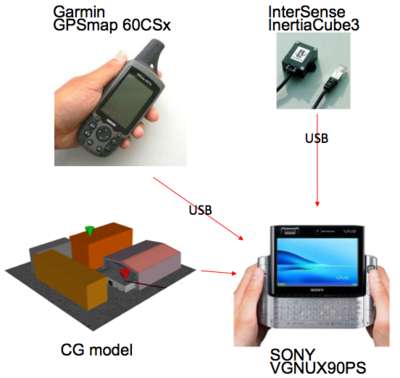
\includegraphics{./Figures/vaio_macbookpro.png}
	\rule{35em}{0.5pt}
	\caption[Prototype architecture]{Prototype architecture}
	\label{fig:VAIOMacBookPro}
\end{figure}

When the user changes the position or orientation of the mobile camera, the video displayed on the screen will simultaneously change accordingly to the camera movement.

The purpose of the above use case is to give an example of the application of visualizing viewing fields of surveillance cameras and to give a rough idea of how the prototype works. There may be other applications. For example, we can build a system which visualizes ``safe paths'' or ``safe areas'' for pupils (figure \ref{fig:HomeSchool}). Pupils can use their cell phones to see if their current location is being well observed when they walk to school or go home from school.

\begin{figure}[htbp]
	\centering
	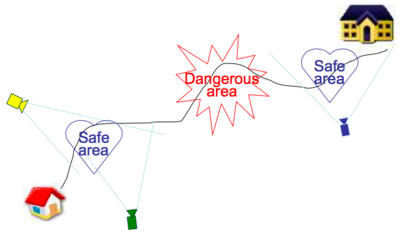
\includegraphics{./Primitives/home_school.png}
	\rule{35em}{0.5pt}
	\caption[Safe path to school]{Safe path to school}
	\label{fig:HomeSchool}
\end{figure}

%------------------------------------------------------------------------------

\section{Background}

For outdoor MR, bulky devices or devices that reduce the mobility of users are not preferable. For example: big computers, devices wired to a fixed position, devices with big auxiliaries, big HMDs, HMDs that prevent users from seeing the outdoor environment while walking\ldots As a result, devices for outdoor MR should be small, lightweight, should connect wirelessly to other devices if they need to.

MR programs usually need to know the position and orientation of the devices in order to merge images of the virtual world to the correct place of the images of the real world. For indoor environment, marker-based solutions are known to work very well \cite{Reference20}. However, outdoor environment is usually large thus it is impossible to put markers everywhere. There have been many researches that use UMPCs equipped with GPS and/or gyrocompass devices \cite{Reference2} \cite{Reference4} \cite{Reference13}. Hardware devices have been becoming smaller and more powerful according to Moore's law. Today's high-end cell phones, like Apple iPhone and Google T-Mobile G1, usually have built-in GPS and accelerometer devices. Because of their small size, high specifications, and competitive prices, such devices have found their use in outdoor MR applications and researches, like Sekai camera \cite{Reference18} and Enkin \cite{Reference19}.

However, normal GPS devices have error of about 5--10 m, and gyrocompass devices suffer from drift error. There have been many researches that are based on the images taken by the camera on the mobile device to deal with this problem. We can follow the approach that uses gravity accelerometer to help eliminate drift error, model-based tracking with edge and texture tracker to help produce accurate localization result \cite{Reference13}. There is also an extreme approach that completely does not require GPS or gyrocompass devices, only uses the images taken by the camera and a landmark database of natural feature points built before-hand \cite{Reference21}.

When MR programs need more memory or CPU power than the mobile devices can provide to run, we have a backup solution in which the mobile devices connect wirelessly to remote non-mobile computers to ask for help. It is possible send realtime video images wirelessly to remote computers for processing because wireless network speed may go up to 54 Mbps. This may be a good approach because Moore's law has slowed down in recent years, thus we cannot expect the specifications of mobile devices to go much higher anytime soon while at the same time keeping their mobility.
